\documentclass[../../main.tex]{subfiles}
\graphicspath{{../../image/}{../../figure/}}
\begin{document}

\section{变分自编码器}\label{section:ch19-变分自编码器}

潜变量模型的似然函数由下式给出：
\begin{align}
p(\bm{x}\mid\bm{w})=\int p(\bm{x}\mid\bm{z},\bm{w})\,p(\bm{z})\,\mathrm{d}\bm{z},
\label{align:ch19-边缘似然}
\end{align}
其中 $p(\bm{x}\mid\bm{z},\bm{w})$ 由一个深度神经网络定义。这个似然函数是难以处理的，因为关于 $\bm{z}$ 的积分无法解析计算。变分自编码器（Variational AutoEncoder，VAE）（Kingma and Welling，2013；Rezende、Mohamed 和 Wierstra，2014；Doersch，2016；Kingma and Welling，2019）在训练模型时使用了这个似然函数的近似表示来解决这一难题。VAE 背后的关键思想如下：
\begin{enumerate}[(1)]
\item 使用证据下界来近似似然函数，从而与 EM 算法形成紧密联系；
\item 借助摊销推断（即使用编码器网络）来近似 E 步骤中潜变量上的后验分布，而不是精确评估每个数据点的后验分布；
\item 使用重参数化（reparameterization）技巧实现编码器模型的可微分训练（参见\cref{section:ch15-em算法}）。
\end{enumerate}

\begin{definition}[变分自编码器]\label{definition:ch19-变分自编码器}
考虑一个生成式模型，其条件分布 $p(\bm{x}\mid\bm{z},\bm{w})$ 覆盖了由深度神经网络输出控制的 $D$ 维数据变量 $\bm{x}$，例如 $\bm{g}(\bm{z},\bm{w})$ 可以表示 Gauss 条件分布的均值。同时考虑 $M$ 维潜变量 $\bm{z}$ 的分布，它由零均值、单位方差的 Gauss 分布给出：
\begin{align}
p(\bm{z})=\mathcal{N}(\bm{z}\mid\bm{0},\bm{I}).
\label{align:ch19-先验}
\end{align}
称以\eqref{align:ch19-边缘似然}为似然、以\eqref{align:ch19-先验}为先验，并用一个编码器网络近似后验 $p(\bm{z}\mid\bm{x},\bm{w})$ 的潜变量模型为\textbf{变分自编码器}（variational autoencoder，VAE）。
\end{definition}

% SUPPLEMENT: parent=definition:ch19-变分自编码器; kind=motivation; location=紧随其后的 remark（重构新增）
\begin{remark}（重构新增）
\cref{definition:ch19-变分自编码器}的出发点是把\cref{chapter:ch16-连续潜变量}中的线性潜变量模型换成非线性模型：$p(\bm{x}\mid\bm{z},\bm{w})$ 不再由矩阵乘法给出，而由深度神经网络给出，因此先验仍然简单（\eqref{align:ch19-先验}），但边缘分布 $p(\bm{x}\mid\bm{w})$ 可以逼近非常复杂的形状。代价是\eqref{align:ch19-边缘似然}的积分不可解：被积函数关于 $\bm{z}$ 的依赖由神经网络决定，既没有闭式原函数，也不能像线性-Gauss 情形那样配方，这正是需要变分近似的根本原因。

逐项说明条件：$D$ 是数据维数，$M$ 是潜空间维数，二者不必相等（通常 $M\ll D$）；先验取标准 Gauss 分布是一个建模选择，它使采样和 KL 项都有闭式表达，但并不是唯一选择，后文的“条件 VAE”就把先验换成 $p(\bm{z}\mid\bm{c})$。$p(\bm{x}\mid\bm{z},\bm{w})$ 的具体形式（Gauss、Bernoulli 等）决定了\eqref{align:ch19-elbo}中被积函数的具体表达式，而本章的推导只用到它的可微性，因此对输出分布的形式并不敏感（参见\cref{section:ch06-混合密度网络}）。
\end{remark}

为了推导出 VAE 的近似，首先回想一下，对于由潜变量 $\bm{z}$ 描述的空间上的任意概率分布 $q(\bm{z})$，以下关系成立（参见\cref{section:ch15-证据下界}）：
\begin{align}
\ln p(\bm{x}\mid\bm{w})=\mathcal{L}(\bm{w})+\operatorname{KL}\big(q(\bm{z})\,\|\,p(\bm{z}\mid\bm{x},\bm{w})\big),
\label{align:ch19-elbo分解}
\end{align}
其中 $\mathcal{L}$ 与 $\operatorname{KL}$ 的定义如下：

\begin{definition}[证据下界与 KL 散度]\label{definition:ch19-证据下界}
设 $q(\bm{z})$ 是潜变量空间上的任意概率密度。称
\begin{align}
\mathcal{L}(\bm{w})=\int q(\bm{z})\ln\Big\{\frac{p(\bm{x}\mid\bm{z},\bm{w})\,p(\bm{z})}{q(\bm{z})}\Big\}\,\mathrm{d}\bm{z}
\label{align:ch19-elbo}
\end{align}
为\textbf{证据下界}（evidence lower bound）或 ELBO，也称\textbf{变分下界}（variational lower bound）。Kullback-Leibler 散度（简称 KL 散度）$\operatorname{KL}(\cdot\,\|\,\cdot)$ 定义为
\begin{align}
\operatorname{KL}\big(q(\bm{z})\,\|\,p(\bm{z}\mid\bm{x},\bm{w})\big)=-\int q(\bm{z})\ln\Big\{\frac{p(\bm{z}\mid\bm{x},\bm{w})}{q(\bm{z})}\Big\}\,\mathrm{d}\bm{z}.
\label{align:ch19-kl}
\end{align}
\end{definition}

% SUPPLEMENT: parent=definition:ch19-证据下界; kind=motivation; location=紧随其后的 remark（重构新增）
\begin{remark}（重构新增）
\cref{definition:ch19-证据下界}中的\eqref{align:ch19-elbo}之所以叫“下界”，马上会由\cref{proposition:ch19-ELBO分解}说明；之所以叫“证据”，是因为在 Bayes 语境中 $\ln p(\bm{x}\mid\bm{w})$ 被称为模型证据（model evidence）。它与\cref{subsection:ch02-KL散度}中的 KL 散度是同一个量，只换成了连续潜变量的积分写法：\eqref{align:ch19-kl}右端的负号使 $\operatorname{KL}\geqslant0$，这与\cref{subsection:ch02-KL散度}的约定一致，因此不能把负号理解成“负的散度”。

这里的 $q(\bm{z})$ 是任意的：它既可以依赖 $\bm{x}$（后文取 $q(\bm{z}\mid\bm{x},\bm{\phi})$），也可以与 $\bm{x}$ 无关。下界对任意 $q$ 都成立，但对不同的 $q$ 松紧不同——$q$ 越接近真实后验 $p(\bm{z}\mid\bm{x},\bm{w})$，下界越紧。这既是变分推断的核心，也是 VAE 中“训练编码器”的目标：编码器的任务就是让 $q$ 逼近后验，从而把下界抬高到接近真实对数似然。最后，两个定义都要求相应的积分存在；若 $q$ 与 $p(\cdot\mid\bm{x},\bm{w})$ 不满足绝对连续性，$\operatorname{KL}$ 取 $+\infty$，\eqref{align:ch19-elbo分解}仍按扩展实数理解。
\end{remark}

\begin{proposition}[证据下界分解]\label{proposition:ch19-ELBO分解}
设 $q(\bm{z})$ 是潜变量空间上的概率密度，且 $\ln p(\bm{x}\mid\bm{w})$ 有限。则\eqref{align:ch19-elbo分解}成立；又因 KL 散度满足 $\operatorname{KL}(q\,\|\,p)\geqslant0$，可以得到
\begin{align}
\ln p(\bm{x}\mid\bm{w})\geqslant\mathcal{L},
\label{align:ch19-elbo下界}
\end{align}
即 $\mathcal{L}$ 是 $\ln p(\bm{x}\mid\bm{w})$ 的证据下界。
\end{proposition}
\begin{proof}（重构新增）
由于 $p(\bm{x}\mid\bm{w})$ 与 $\bm{z}$ 无关，且 $\int q(\bm{z})\,\mathrm{d}\bm{z}=1$，有
\begin{align*}
\ln p(\bm{x}\mid\bm{w})&=\int q(\bm{z})\ln p(\bm{x}\mid\bm{w})\,\mathrm{d}\bm{z}\\
&=\int q(\bm{z})\ln\frac{p(\bm{x},\bm{z}\mid\bm{w})}{p(\bm{z}\mid\bm{x},\bm{w})}\,\mathrm{d}\bm{z}\\
&=\int q(\bm{z})\ln\Big\{\frac{p(\bm{x}\mid\bm{z},\bm{w})\,p(\bm{z})}{q(\bm{z})}\Big\}\,\mathrm{d}\bm{z}-\int q(\bm{z})\ln\Big\{\frac{p(\bm{z}\mid\bm{x},\bm{w})}{q(\bm{z})}\Big\}\,\mathrm{d}\bm{z}\\
&=\mathcal{L}(\bm{w})+\operatorname{KL}\big(q(\bm{z})\,\|\,p(\bm{z}\mid\bm{x},\bm{w})\big),
\end{align*}
其中第三步把 $\ln\{p(\bm{x},\bm{z}\mid\bm{w})/p(\bm{z}\mid\bm{x},\bm{w})\}$ 拆成 $\ln\{p(\bm{x}\mid\bm{z},\bm{w})p(\bm{z})/q(\bm{z})\}-\ln\{p(\bm{z}\mid\bm{x},\bm{w})/q(\bm{z})\}$，两处都用了 Bayes 定理 $p(\bm{x},\bm{z}\mid\bm{w})=p(\bm{x}\mid\bm{z},\bm{w})p(\bm{z})=p(\bm{z}\mid\bm{x},\bm{w})p(\bm{x}\mid\bm{w})$。第四步按\eqref{align:ch19-elbo}与\eqref{align:ch19-kl}的定义。由于对任意两个概率密度有 $\operatorname{KL}\geqslant0$，由\eqref{align:ch19-elbo分解}立得\eqref{align:ch19-elbo下界}。
\end{proof}

% SUPPLEMENT: parent=proposition:ch19-ELBO分解; kind=motivation; location=紧随其后的 remark（重构新增）
\begin{remark}（重构新增）
\cref{proposition:ch19-ELBO分解}给出了一条清晰的改进路径：对数似然固定，因此“抬高下界”与“缩小 KL”是同一件事。EM 算法之所以能让下界最终等于对数似然，是因为它取 $q$ 为精确后验，使 KL 恰为零；VAE 中 $q$ 被限制在一个神经网络参数化的分布族里，KL 一般不为零，这就留下了原书后文所说的“残差”。

证明只用到 Bayes 定理与 $\int q=1$，因此结论对任意 $q$ 成立，并不要求 $q$ 是 Gauss 分布或因子分解的。条件“$\ln p(\bm{x}\mid\bm{w})$ 有限”用于避免 $\infty-\infty$；若 $q$ 在 $p(\bm{z}\mid\bm{x},\bm{w})=0$ 的区域为正，KL 为 $+\infty$，此时\eqref{align:ch19-elbo分解}应理解为扩展实数等式，下界自动失效。这也解释了为什么编码器的输出方差必须保持为正：若某个 $\sigma_j\to0$，KL 中的 $-\ln\sigma_j^{2}$ 会发散，下界随之失去意义。
\end{remark}

所以 $\mathcal{L}$ 是 $\ln p(\bm{x}\mid\bm{w})$ 的证据下界。虽然对数似然函数 $\ln p(\bm{x}\mid\bm{w})$ 难以直接计算，但我们可以使用 Monte Carlo 估计方法来评估这个下界，从而使它近似于真实对数似然函数的值。

考虑从模型分布 $p(\bm{x})$ 中独立采样的训练数据集 $\mathcal{D}=\{\bm{x}_1,\cdots,\bm{x}_N\}$。这个数据集的对数似然函数由下式给出：
\begin{align}
\ln p(\mathcal{D}\mid\bm{w})=\sum_{n=1}^{N}\mathcal{L}_n+\sum_{n=1}^{N}\operatorname{KL}\big(q_n(\bm{z}_n)\,\|\,p(\bm{z}_n\mid\bm{x}_n,\bm{w})\big),
\label{align:ch19-总elbo}
\end{align}
其中
\begin{align}
\mathcal{L}_n=\int q_n(\bm{z}_n)\ln\Big\{\frac{p(\bm{x}_n\mid\bm{z}_n,\bm{w})\,p(\bm{z}_n)}{q_n(\bm{z}_n)}\Big\}\,\mathrm{d}\bm{z}_n.
\label{align:ch19-逐点elbo}
\end{align}

请注意，这引入了与每个数据向量 $\bm{x}_n$ 相对应的单独潜变量 $\bm{z}_n$，就像我们在混合模型和概率 PCA 模型中看到的那样。因此，每个潜变量都有自己的独立分布 $q_n(\bm{z}_n)$，且都可以单独优化（参见\cref{section:ch15-Gauss混合分布}和\cref{section:ch16-概率潜变量}）。

由于\eqref{align:ch19-总elbo}对任意选取的分布 $q_n(\bm{z})$ 都成立，我们可以选择能使下限 $\mathcal{L}_n$ 最大化的分布，或等价地选择最小化 KL 散度 $\operatorname{KL}(q_n(\bm{z}_n)\|p(\bm{z}_n\mid\bm{x}_n,\bm{w}))$ 的分布。在先前的简单 Gauss 混合模型和概率 PCA 模型中，我们可以在 EM 算法的 E 步骤中精确计算这些后验分布，即将每个 $q_n(\bm{z}_n)$ 设置为相应的后验分布 $p(\bm{z}_n\mid\bm{x}_n,\bm{w})$。此时 KL 散度降为 $0$，因此下界等于真实的对数似然。\cref{figure:ch19-后验分布}使用我们之前在生成对抗网络相关章节所举的简单例子解释了后验分布（参见\cref{subsection:ch16-非线性流形}）。

$\bm{z}_n$ 的精确后验分布由 Bayes 定理给出：
\begin{align}
p(\bm{z}_n\mid\bm{x}_n,\bm{w})=\frac{p(\bm{x}_n\mid\bm{z}_n,\bm{w})\,p(\bm{z}_n)}{p(\bm{x}_n\mid\bm{w})}.
\label{align:ch19-后验}
\end{align}

\begin{figure}[htbp]
\centering
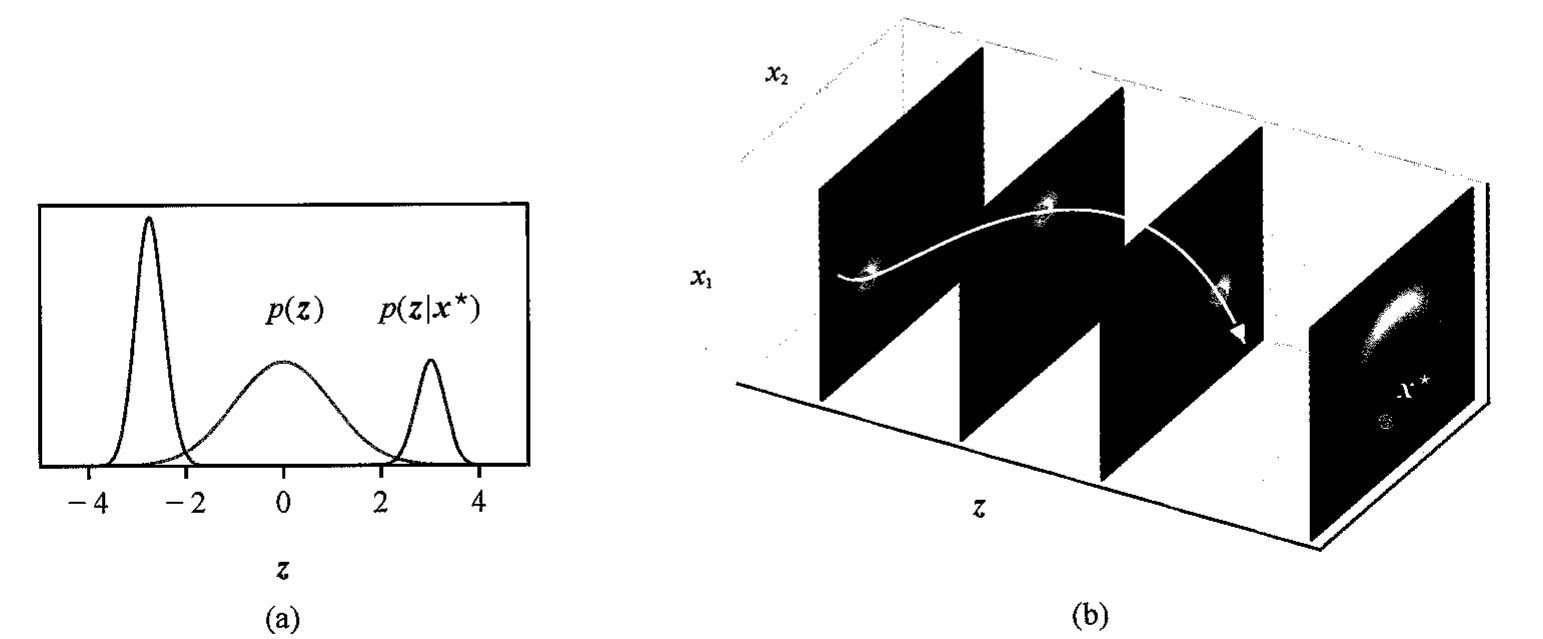
\includegraphics[width=0.85\textwidth]{ch19-fig516-posterior.png}
\caption{与\cref{figure:ch16-非线性潜变量示意}相似，计算非线性潜变量模型的后验分布。边缘分布 $p(\bm{x})$ 显示在 (b) 的最右侧图中，其具有香蕉形状，数据点 $\bm{x}^{*}$ 更接近香蕉形状的尖端。后验分布 $p(\bm{z}\mid\bm{x}^{*})$ 显示在 (a) 中，它是双模态的，即使先验分布 $p(\bm{z})$ 是单模态的 [来源于 Prince (2020)，经授权使用]}
\label{figure:ch19-后验分布}
\end{figure}

对于深度生成式模型，\eqref{align:ch19-后验}中的分子是可以直接计算的。然而分母是由似然函数给出的，难以解析计算。因此，我们需要找到一个对后验分布的近似。原则上，我们可以考虑为每个分布 $q_n(\bm{z}_n)$ 单独建立参数化模型，并进行数值优化，但计算成本非常高，特别是对于大数据集来说，此外还需要在每次更新 $\bm{w}$ 后重新计算分布。因此，我们决定换一个方向，引入第二个神经网络来探索一个更有效的近似框架。

\subsection{摊销推理}\label{subsection:ch19-摊销推理}

在变分自编码器中，我们不再单独为每个数据点 $\bm{x}_n$ 计算一个后验分布 $p(\bm{z}_n\mid\bm{x}_n,\bm{w})$，而是通过训练一个称为编码器网络的神经网络来近似所有这些分布。

\begin{definition}[摊销推理与编码器网络]\label{definition:ch19-摊销推理}
用单个以 $\bm{x}$ 为输入、以 $\bm{\phi}$ 为参数的神经网络输出条件分布 $q(\bm{z}\mid\bm{x},\bm{\phi})$，并用它同时近似所有数据点的后验分布 $p(\bm{z}_n\mid\bm{x}_n,\bm{w})$，这种技术称为\textbf{摊销推理}（amortized inference），该神经网络称为\textbf{编码器网络}（encoder network），$\bm{\phi}$ 称为\textbf{编码器参数}。
\end{definition}

% SUPPLEMENT: parent=definition:ch19-摊销推理; kind=motivation; location=紧随其后的 remark（重构新增）
\begin{remark}（重构新增）
\cref{definition:ch19-摊销推理}中“摊销”一词来自计算成本的分摊：逐个数据点优化 $q_n$ 的代价是每个数据点都要单独做一次优化，且每次更新 $\bm{w}$ 后旧结果全部作废；摊销推理把这份代价一次性“摊”到一个共享的编码器上——训练一次，之后对任何 $\bm{x}$ 只需一次前向传播就能得到近似后验。代价是表达能力受限：一个网络必须同时拟合所有数据点的后验，遇到多模态或强非 Gauss 的后验时只能给出平均意义上的近似（见\cref{figure:ch19-后验分布}中双模态的例子）。

条件方面：$q$ 必须以 $\bm{x}$ 为条件（否则退化为与数据无关的先验，即后文的“后验崩塌”）；$\bm{\phi}$ 与解码器参数 $\bm{w}$ 相互独立，才能联合优化；摊销推理本身并不要求 $q$ 是 Gauss 分布，只要求它可采样、可求 KL 或可估计其梯度——第（3）点“重参数化”正是为此服务。
\end{remark}

由证据下界给出的目标函数现在同时依赖于 $\bm{\phi}$ 和 $\bm{w}$，我们可以使用基于梯度的优化方法来联合优化这两组参数。

因此，VAE 包含两个参数独立但能联合训练的神经网络：一个编码器网络，用于将数据向量映射到潜空间；一个解码器网络，用于将潜空间向量映射回数据空间。这类似于简单的神经网络自编码器模型，所不同的是，我们在潜空间中定义了一个概率分布。我们将看到，编码器根据 Bayes 定理计算解码器的近似概率逆过程——即根据给定观测数据推断潜变量的分布。

\begin{definition}[对角 Gauss 编码器]\label{definition:ch19-对角Gauss编码器}
在变分自编码器中，编码器的一个典型选择是具有对角协方差矩阵的 Gauss 分布，其均值 $\mu_j$ 和方差 $\sigma_j^{2}$ 由一个以 $\bm{x}$ 作为输入的神经网络给出：
\begin{align}
q(\bm{z}\mid\bm{x},\bm{\phi})=\prod_{j=1}^{M}\mathcal{N}\big(z_j\mid\mu_j(\bm{x},\bm{\phi}),\,\sigma_j^{2}(\bm{x},\bm{\phi})\big).
\label{align:ch19-编码器}
\end{align}
\end{definition}

% SUPPLEMENT: parent=definition:ch19-对角Gauss编码器; kind=motivation; location=紧随其后的 remark（重构新增）
\begin{remark}（重构新增）
\cref{definition:ch19-对角Gauss编码器}选择因子分解的 Gauss 分布有两个直接好处：其一，$q$ 与标准 Gauss 先验之间的 KL 有闭式\eqref{align:ch19-klGauss}，无需 Monte Carlo；其二，采样只需 $M$ 个独立的一维 Gauss 样本，重参数化\eqref{align:ch19-重参数化采样}逐分量成立。代价是排除了后验各分量之间的相关性，原书后文列出的“真实后验未必服从因子分解的 Gauss 分布”正是这一限制；\cref{exercise:ch19-03}给出了用下三角矩阵 $\bm{L}$ 引入一般协方差矩阵的推广。

注意 $\mu_j(\bm{x},\bm{\phi})$ 取值于 $(-\infty,\infty)$，而 $\sigma_j^{2}(\bm{x},\bm{\phi})$ 必须非负，所以两者的输出单元不能用同一种激活函数：前者可以用线性单元，后者通常用指数函数 $\exp(\cdot)$ 以保证为正。用 $\exp$ 的代价是数值上可能溢出，实践中常改用 softplus 或对 $\ln\sigma_j^{2}$ 直接建模。
\end{remark}

请注意，均值 $\mu_j(\bm{x},\bm{\phi})$ 位于区间 $(-\infty,\infty)$，因此相应的输出单元激活函数可以是线性的；而方差 $\sigma_j^{2}(\bm{x},\bm{\phi})$ 必须是非负的，所以相关的输出单元通常使用指数函数 $\exp(\cdot)$ 作为激活函数。

我们的优化目标是使用基于梯度的优化方法，针对参数 $\bm{\phi}$ 和 $\bm{w}$ 最大化这个下界，这通常使用基于小批量数据的随机梯度下降法来实现。尽管是联合优化参数，但从概念上我们可以交替地优化 $\bm{\phi}$ 和 $\bm{w}$，如\cref{figure:ch19-elbo优化}所示。

\begin{figure}[htbp]
\centering
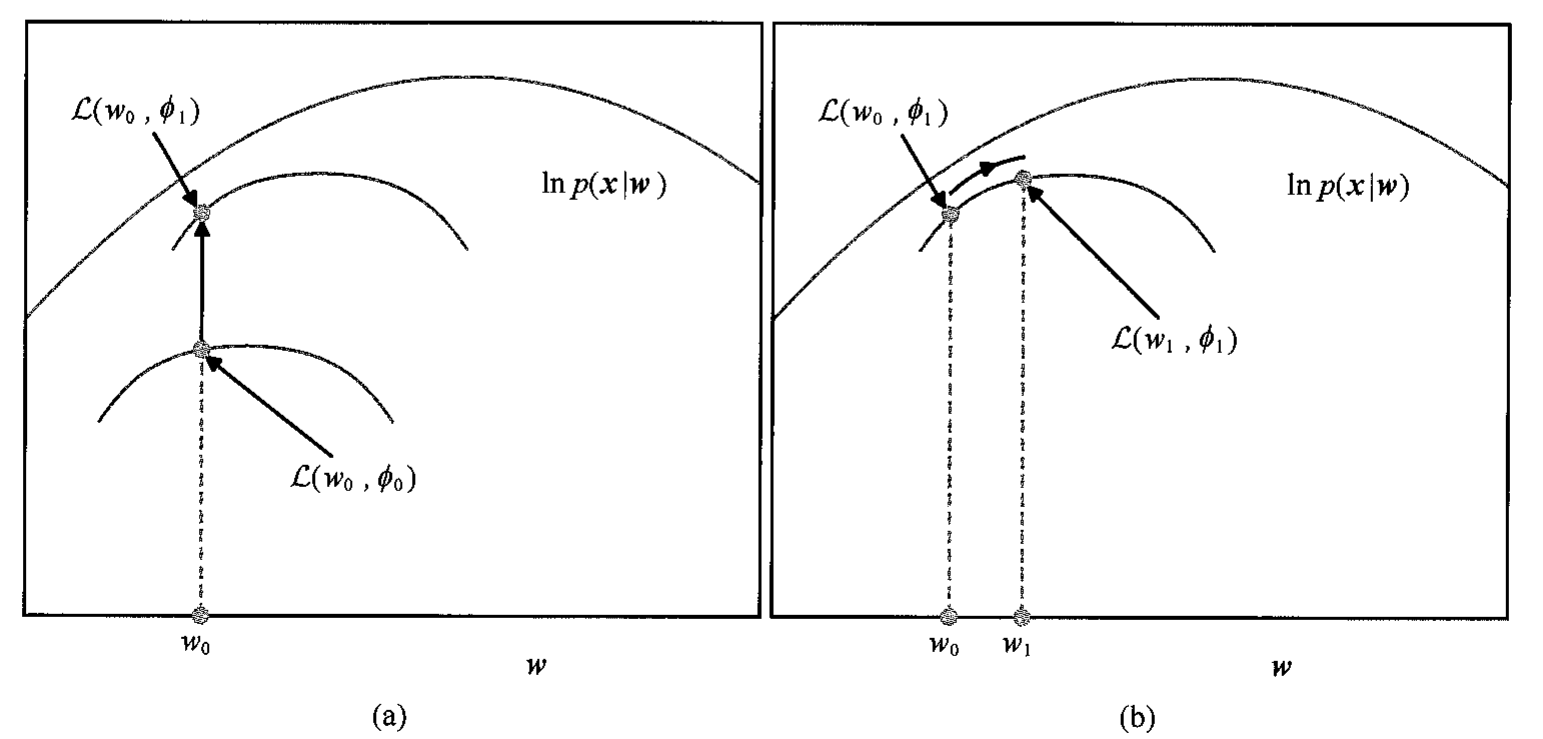
\includegraphics[width=0.82\textwidth]{ch19-fig517-elbo-opt.png}
\caption{对证据下界（ELBO）进行优化的示意图。(a) 对于解码器网络参数 $\bm{w}$ 的给定值 $\bm{w}_0$，我们可以通过优化编码器网络的参数 $\bm{\phi}$ 来提高这个下界的值。(b) 对于给定的 $\bm{\phi}$ 值，我们可以通过优化 $\bm{w}$ 来增大 ELBO 函数的值。请注意，蓝色曲线所示的 ELBO 函数始终位于红色曲线所示的对数似然函数之下，这是因为编码器网络通常无法完全匹配真实的后验分布}
\label{figure:ch19-elbo优化}
\end{figure}

ELBO 优化与 EM 算法的一个关键区别是，对于给定的 $\bm{w}$ 值，相对于编码器参数 $\bm{\phi}$ 的优化通常不会将 KL 散度降低到零，因为编码器网络并不能完美地预测后验潜在分布，所以下界和真实对数似然之间仍然存在残差。尽管基于深度神经网络的编码器非常灵活，但它并不能精确地模拟真实的后验分布，原因如下：
\begin{enumerate}[(1)]
\item 真实的条件后验分布未必服从因子分解的 Gauss 分布；
\item 即使是一个大型神经网络，也存在灵活性方面的限制；
\item 训练过程只是一个近似的优化。
\end{enumerate}
\cref{figure:ch19-em与elbo}对 EM 算法和 ELBO 优化之间的关系做了总结。

\begin{figure}[htbp]
\centering
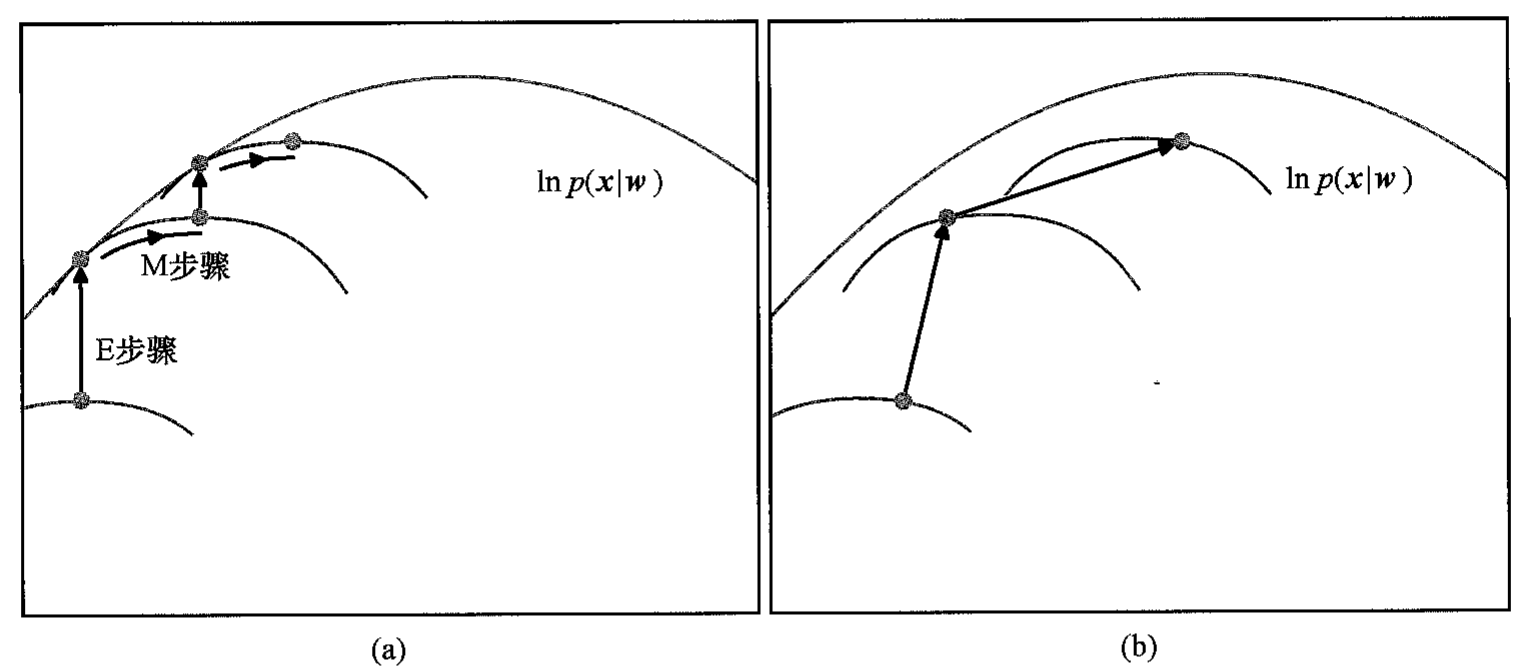
\includegraphics[width=0.85\textwidth]{ch19-fig518-em-elbo.png}
\caption{EM 算法和 ELBO 优化之间的关系。(a) 在 EM 算法中，我们在 E 步骤中交替更新变分后验分布，并在 M 步骤中更新模型参数。E 步骤是精确的，在每个 E 步骤之后，下界与对数似然之间的差距将减小到零。(b) 在 ELBO 优化中，我们执行的是编码器网络参数 $\bm{\phi}$（类似于 E 步骤）和解码器网络参数 $\bm{w}$（类似于 M 步骤）的联合优化}
\label{figure:ch19-em与elbo}
\end{figure}

\subsection{重参数化技巧}\label{subsection:ch19-重参数化}

遗憾的是，到目前为止，下界 [式\eqref{align:ch19-逐点elbo}] 仍然难以直接计算，因为在潜变量 $\bm{z}$ 的积分过程中，解码器网络会导致被积函数对潜变量存在复杂的依赖关系。对于数据点 $\bm{x}_n$，其对下界的贡献可以表示为：
\begin{align}
\mathcal{L}_n(\bm{w},\bm{\phi})&=\int q(\bm{z}_n\mid\bm{x}_n,\bm{\phi})\ln\Big\{\frac{p(\bm{x}_n\mid\bm{z}_n,\bm{w})\,p(\bm{z}_n)}{q(\bm{z}_n\mid\bm{x}_n,\bm{\phi})}\Big\}\mathrm{d}\bm{z}_n\label{align:ch19-逐点elbo拆分}\\
&=\int q(\bm{z}_n\mid\bm{x}_n,\bm{\phi})\ln p(\bm{x}_n\mid\bm{z}_n,\bm{w})\,\mathrm{d}\bm{z}_n-\operatorname{KL}\big(q(\bm{z}_n\mid\bm{x}_n,\bm{\phi})\,\|\,p(\bm{z}_n)\big).\nonumber
\end{align}

\eqref{align:ch19-逐点elbo拆分}右侧的第二项是两个 Gauss 分布之间的 KL 散度，并且可以解析评估（见\cref{exercise:ch02-27}）：
\begin{align}
\operatorname{KL}\big(q(\bm{z}_n\mid\bm{x}_n,\bm{\phi})\,\|\,p(\bm{z}_n)\big)=\frac{1}{2}\sum_{j=1}^{M}\Big\{1+\ln\sigma_j^{2}(\bm{x}_n)-\mu_j^{2}(\bm{x}_n)-\sigma_j^{2}(\bm{x}_n)\Big\}.
\label{align:ch19-klGauss}
\end{align}

\begin{remark}（重构新增）原文问题说明：\eqref{align:ch19-klGauss}的右端按\eqref{align:ch19-kl}的符号约定并不等于左端的 KL 散度，而是它的相反数。由\cref{exercise:ch19-04}的直接计算，
\begin{align*}
\operatorname{KL}\big(\mathcal{N}(\mu,\sigma^{2})\,\|\,\mathcal{N}(0,1)\big)=\frac{1}{2}\Big(\mu^{2}+\sigma^{2}-1-\ln\sigma^{2}\Big)\geqslant0,
\end{align*}
把 $-\operatorname{KL}$ 代入\eqref{align:ch19-逐点elbo拆分}，即得
\begin{align*}
-\operatorname{KL}\big(q(\bm{z}_n\mid\bm{x}_n,\bm{\phi})\,\|\,p(\bm{z}_n)\big)=\frac{1}{2}\sum_{j=1}^{M}\Big\{1+\ln\sigma_j^{2}(\bm{x}_n)-\mu_j^{2}(\bm{x}_n)-\sigma_j^{2}(\bm{x}_n)\Big\},
\end{align*}
这正是\eqref{align:ch19-klGauss}的右端。因此\eqref{align:ch19-klGauss}应读作“$-\operatorname{KL}$ 的闭式”，或把花括号内的符号整体取反；后文\eqref{align:ch19-完整损失}正是以 $-\operatorname{KL}$ 的形式使用它的，故损失函数的写法与标准的 ELBO 一致，只有\eqref{align:ch19-klGauss}这一行少了一个负号。若直接按左端为 KL 使用，会得到“KL 可以取负值”的矛盾结论，与\eqref{align:ch19-elbo下界}所依赖的 $\operatorname{KL}\geqslant0$ 冲突。
\end{remark}

对于\eqref{align:ch19-逐点elbo拆分}，我们可以尝试用一个简单的 Monte Carlo 估计法来近似潜变量 $\bm{z}_n$ 上的积分：
\begin{align}
\int q(\bm{z}_n\mid\bm{x}_n,\bm{\phi})\ln p(\bm{x}_n\mid\bm{z}_n,\bm{w})\,\mathrm{d}\bm{z}_n\approx\frac{1}{L}\sum_{l=1}^{L}\ln p(\bm{x}_n\mid\bm{z}_n^{(l)},\bm{w}),
\label{align:ch19-蒙特卡洛}
\end{align}
其中 $\bm{z}_n^{(l)}$ 是从编码器分布 $q(\bm{z}_n\mid\bm{x}_n,\bm{\phi})$ 中采样。关于 $\bm{w}$ 求导很容易，但关于 $\bm{\phi}$ 求梯度却存在问题，因为参数 $\bm{\phi}$ 的变化也会改变采样分布 $q(\bm{z}_n\mid\bm{x}_n,\bm{\phi})$。然而这些样本是固定值，所以我们没有办法获取这些样本相对于 $\bm{\phi}$ 的导数。从概念上讲，我们可以认为将潜变量 $\bm{z}_n$ 固定到特定样本值的过程阻止了误差信号向编码器网络的反向传播，如\cref{figure:ch19-重参数化阻断}所示。

\begin{figure}[htbp]
\centering
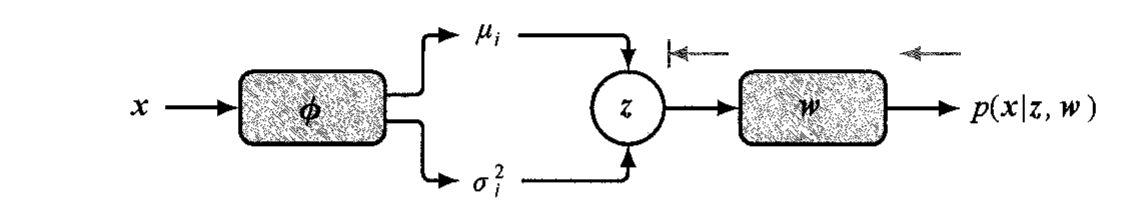
\includegraphics[width=0.78\textwidth]{ch19-fig519-reparam-block.png}
\caption{将潜变量 $\bm{z}$ 固定到特定采样值的过程阻止了误差信号向编码器网络的反向传播}
\label{figure:ch19-重参数化阻断}
\end{figure}

我们可以使用重参数化技巧来解决这个问题。重新设计 Monte Carlo 采样过程，以便明确计算相对于 $\bm{\phi}$ 的导数。

\begin{definition}[重参数化技巧]\label{definition:ch19-重参数化}
设 $q(\bm{z}\mid\bm{x},\bm{\phi})$ 是由参数 $\bm{\phi}$ 指定的一族分布。若存在与 $\bm{\phi}$ 无关的随机变量 $\bm{\varepsilon}$（其分布 $p(\bm{\varepsilon})$ 与 $\bm{\phi}$ 无关）以及关于 $\bm{\phi}$ 可微的映射 $\bm{z}=h(\bm{\varepsilon};\bm{\phi})$，使得当 $\bm{\varepsilon}\sim p(\bm{\varepsilon})$ 时 $h(\bm{\varepsilon};\bm{\phi})$ 服从 $q(\bm{z}\mid\bm{x},\bm{\phi})$，则称用这种“先采样 $\bm{\varepsilon}$、再作确定性变换”的方式实现 $q$ 的采样为\textbf{重参数化}（reparameterization），并称之为\textbf{重参数化技巧}（reparameterization trick）。
\end{definition}

% SUPPLEMENT: parent=definition:ch19-重参数化; kind=motivation; location=紧随其后的 remark（重构新增）
\begin{remark}（重构新增）
\cref{definition:ch19-重参数化}的要点是把“随机性”与“参数依赖性”分离：随机性全部交给与 $\bm{\phi}$ 无关的 $\bm{\varepsilon}$，而 $\bm{\phi}$ 只出现在确定性的变换 $h$ 中。这样样本 $\bm{z}^{(l)}=h(\bm{\varepsilon}^{(l)};\bm{\phi})$ 就是 $\bm{\phi}$ 的可微函数，梯度可以沿 $h$ 反传到编码器，而不必对采样过程本身求导——\cref{figure:ch19-重参数化阻断}中被切断的反向通路因此重新连通（见\cref{figure:ch19-重参数化流}）。

适用条件是本质性的：$h$ 必须存在且可微。对连续分布，这通常可以做到（如 Gauss 用 $h(\varepsilon;\phi)=\mu+\sigma\varepsilon$）；对离散分布则不存在这样的可微变换，这正是重参数化技巧“仅限于连续变量上的分布”的原因。此外，$\bm{\varepsilon}$ 的分布必须与 $\bm{\phi}$ 无关，否则“分离随机性”就无从谈起；若 $q$ 的支撑随 $\bm{\phi}$ 变化（例如均匀分布的区间端点依赖 $\bm{\phi}$），$h$ 仍可构造，但需要显式处理端点。
\end{remark}

首先请注意，如果 $\bm{\varepsilon}$ 是一个均值为零且方差为单位方差的 Gauss 随机变量，那么：

\begin{proposition}[重参数化采样的分布]\label{proposition:ch19-重参数化分布}
设 $\varepsilon$ 具有均值为零、方差为单位方差的 Gauss 分布，$\mu\in\mathbb{R}$、$\sigma>0$。定义
\begin{align}
z=\sigma\varepsilon+\mu,
\label{align:ch19-重参数化采样}
\end{align}
则 $z$ 具有均值为 $\mu$、方差为 $\sigma^{2}$ 的 Gauss 分布（见\cref{exercise:ch19-02}）。
\end{proposition}
\begin{proof}（重构新增）
记 $\varepsilon\sim\mathcal{N}(0,1)$ 的分布函数为 $\Phi$、密度为 $\varphi$。对任意 $t\in\mathbb{R}$，
\begin{align*}
F_z(t)=\mathbb{P}(z\leqslant t)=\mathbb{P}\Big(\varepsilon\leqslant\frac{t-\mu}{\sigma}\Big)=\Phi\Big(\frac{t-\mu}{\sigma}\Big),
\end{align*}
其中第二个等号用了 $\sigma>0$（故不等式方向不变）。对 $t$ 求导，由链式法则
\begin{align*}
f_z(t)=\frac{1}{\sigma}\varphi\Big(\frac{t-\mu}{\sigma}\Big)=\frac{1}{\sqrt{2\pi}\,\sigma}\exp\Big\{-\frac{(t-\mu)^{2}}{2\sigma^{2}}\Big\},
\end{align*}
这正是 $\mathcal{N}(\mu,\sigma^{2})$ 的密度。又 $\mathbb{E}[z]=\sigma\mathbb{E}[\varepsilon]+\mu=\mu$，$\operatorname{Var}(z)=\sigma^{2}\operatorname{Var}(\varepsilon)=\sigma^{2}$。
\end{proof}

% SUPPLEMENT: parent=proposition:ch19-重参数化分布; kind=motivation; location=紧随其后的 remark（重构新增）
\begin{remark}（重构新增）
\cref{proposition:ch19-重参数化分布}是重参数化技巧的算术基础：它保证“先采 $\varepsilon$ 再作线性变换”得到的样本与“直接从 $q$ 采样”同分布，因此可以放心地把样本写成 $\bm{\phi}$ 的可微函数。条件 $\sigma>0$ 不能去掉：若 $\sigma=0$，$z\equiv\mu$ 是退化分布，分布函数在 $t=\mu$ 处跳跃，上面的求导不再成立，此时应按退化分布理解（采样结果与 $\bm{\phi}$ 的依赖仍然可微，只是不再有密度）。多维情形逐分量成立，因为对角 Gauss 的各分量独立。

原书把它留作\cref{exercise:ch19-02}，是为了让读者亲手验证“仿射变换保持 Gaussian 性”这一事实；更一般的线性变换 $z=\mu+L\varepsilon$ 的协方差是 $LL^{\mathsf T}$，见\cref{exercise:ch19-03}。
\end{remark}

$z$ 将具有均值为 $\mu$、方差为 $\sigma^{2}$ 的 Gauss 分布（见\cref{exercise:ch19-02}）。将其应用于\eqref{align:ch19-蒙特卡洛}中的采样过程，其中 $\mu$ 和 $\sigma$ 由编码器网络的输出 $\mu_j(\bm{x}_n,\bm{\phi})$ 和 $\sigma_j^{2}(\bm{x}_n,\bm{\phi})$ 确定，分别对应于\eqref{align:ch19-编码器}的均值和方差。我们不直接从潜变量 $\bm{z}_n$ 采样，而是对 $\bm{\varepsilon}$ 采样，并使用\eqref{align:ch19-重参数化采样}计算对应的 $\bm{z}_n$ 样本：
\begin{align}
z_{nj}^{(l)}=\mu_j(\bm{x}_n,\bm{\phi})\,\varepsilon_{nj}^{(l)}+\sigma_j^{2}(\bm{x}_n,\bm{\phi}).
\label{align:ch19-重参数化样本}
\end{align}

\begin{remark}（重构新增）原文问题说明：\eqref{align:ch19-重参数化样本}与\eqref{align:ch19-重参数化采样}不一致。按\eqref{align:ch19-重参数化采样}，第 $j$ 个分量应为
\begin{align*}
z_{nj}^{(l)}=\mu_j(\bm{x}_n,\bm{\phi})+\sigma_j(\bm{x}_n,\bm{\phi})\,\varepsilon_{nj}^{(l)},
\end{align*}
即 $\mu_j$ 与 $\varepsilon_{nj}^{(l)}$ 是相加关系、乘在 $\varepsilon$ 上的是标准差 $\sigma_j$ 而不是方差 $\sigma_j^{2}$。\eqref{align:ch19-重参数化样本}若按字面理解，得到的 $z_{nj}$ 的方差将是 $\mu_j^{2}$ 而非 $\sigma_j^{2}$，与\eqref{align:ch19-编码器}所定义的 $q$ 不符；把它代入\eqref{align:ch19-完整损失}也会使 KL 项与重构项不再对应同一个分布。原书随后在\eqref{align:ch19-完整损失}下方给出的元素表达式 $z_{nj}^{(l)}=\sigma_{nj}\varepsilon^{(l)}+\mu_{nj}$（其中 $\sigma_{nj}=\sigma_j(\bm{x}_n,\bm{\phi})$）正是上面的正确形式，可作为内部一致的依据；算法 19.1 中同一行赋值也应按此更正。本译本保留原式以供对照，实际使用时应采用修正形式。
\end{remark}

其中 $l=1,\cdots,L$ 是样本的索引。该方法显式建立 $\bm{\phi}$ 与采样值之间的依赖关系，使梯度计算可行，如\cref{figure:ch19-重参数化流}所示。

\begin{figure}[htbp]
\centering
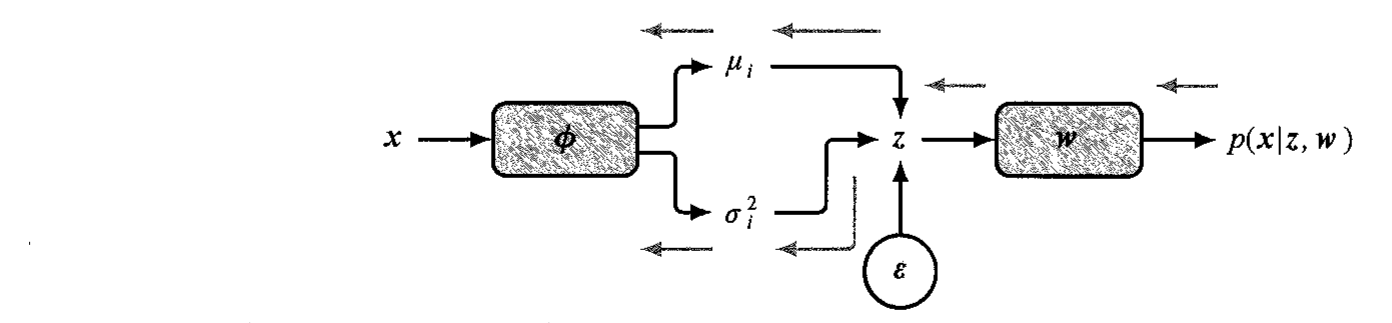
\includegraphics[width=0.85\textwidth]{ch19-fig519-reparam-flow.png}
\caption{重参数化技巧通过对一个独立随机变量 $\bm{\varepsilon}$ 的样本进行计算而不是直接采样 $\bm{z}$，从而允许误差信号反向传播到编码器网络。得到的模型可以使用基于梯度的优化来学习编码器网络和解码器网络的参数}
\label{figure:ch19-重参数化流}
\end{figure}

重参数化技巧可以扩展到其他分布，但仅限于连续变量上的分布。有的估计器可以直接计算梯度而无须使用重参数化技巧（Williams，1992），但这些估计器的方差很大，因此重参数化技巧也可以看作一种有效的方差降低技术。

\begin{proposition}[重参数化梯度估计的无偏性（重构新增）]\label{proposition:ch19-重参数化梯度}
设 $q(\bm{z}\mid\bm{x},\bm{\phi})=\mathcal{N}\big(\bm{z}\mid\bm{\mu}(\bm{x},\bm{\phi}),\operatorname{diag}(\bm{\sigma}^{2}(\bm{x},\bm{\phi}))\big)$，$\bm{z}=\bm{\mu}(\bm{x},\bm{\phi})+\bm{\sigma}(\bm{x},\bm{\phi})\odot\bm{\varepsilon}$，$\bm{\varepsilon}\sim\mathcal{N}(\bm{0},\bm{I})$。设 $\ln p(\bm{x}\mid\bm{z},\bm{w})$ 关于 $\bm{z}$ 连续可微，且存在与 $\bm{\phi}$ 无关的可积控制函数 $g(\bm{\varepsilon})$ 使得 $\|\nabla_{\bm{\phi}}\ln p(\bm{x}\mid\bm{\mu}(\bm{x},\bm{\phi})+\bm{\sigma}(\bm{x},\bm{\phi})\odot\bm{\varepsilon},\bm{w})\|\leqslant g(\bm{\varepsilon})$，则
\begin{align*}
\nabla_{\bm{\phi}}\mathbb{E}_{q(\bm{z}\mid\bm{x},\bm{\phi})}\big[\ln p(\bm{x}\mid\bm{z},\bm{w})\big]=\mathbb{E}_{\bm{\varepsilon}\sim\mathcal{N}(\bm{0},\bm{I})}\big[\nabla_{\bm{\phi}}\ln p\big(\bm{x}\mid\bm{\mu}(\bm{x},\bm{\phi})+\bm{\sigma}(\bm{x},\bm{\phi})\odot\bm{\varepsilon},\bm{w}\big)\big],
\end{align*}
即用 $\bm{\varepsilon}$ 的样本对右端作 Monte Carlo 平均，得到左端梯度的无偏估计。
\end{proposition}
\begin{proof}（重构新增）
记 $\bm{z}(\bm{\varepsilon};\bm{\phi})=\bm{\mu}(\bm{x},\bm{\phi})+\bm{\sigma}(\bm{x},\bm{\phi})\odot\bm{\varepsilon}$。由\cref{proposition:ch19-重参数化分布}（逐分量），当 $\bm{\varepsilon}\sim\mathcal{N}(\bm{0},\bm{I})$ 时 $\bm{z}(\bm{\varepsilon};\bm{\phi})\sim q(\bm{z}\mid\bm{x},\bm{\phi})$，故对任意可积的 $F$，
\begin{align*}
\mathbb{E}_{q(\bm{z}\mid\bm{x},\bm{\phi})}[F(\bm{z})]=\mathbb{E}_{\bm{\varepsilon}}[F(\bm{z}(\bm{\varepsilon};\bm{\phi}))].
\end{align*}
取 $F(\bm{z})=\ln p(\bm{x}\mid\bm{z},\bm{w})$。右端的被积函数关于 $\bm{\phi}$ 可微，且由控制函数条件可在积分号下求导，于是
\begin{align*}
\nabla_{\bm{\phi}}\mathbb{E}_{q}[F]&=\nabla_{\bm{\phi}}\int F\big(\bm{z}(\bm{\varepsilon};\bm{\phi})\big)p(\bm{\varepsilon})\,\mathrm{d}\bm{\varepsilon}\\
&=\int\nabla_{\bm{z}}F\big(\bm{z}(\bm{\varepsilon};\bm{\phi})\big)^{\mathsf T}\,\nabla_{\bm{\phi}}\bm{z}(\bm{\varepsilon};\bm{\phi})\,p(\bm{\varepsilon})\,\mathrm{d}\bm{\varepsilon}\\
&=\mathbb{E}_{\bm{\varepsilon}}\Big[\nabla_{\bm{\phi}}\ln p\big(\bm{x}\mid\bm{\mu}(\bm{x},\bm{\phi})+\bm{\sigma}(\bm{x},\bm{\phi})\odot\bm{\varepsilon},\bm{w}\big)\Big],
\end{align*}
其中第二个等号是链式法则，第三个等号把对 $\bm{\phi}$ 的全导数写成 $\nabla_{\bm{\phi}}\ln p(\bm{x}\mid\bm{z}(\bm{\varepsilon};\bm{\phi}),\bm{w})$。用 $L$ 个独立样本平均即得无偏估计，其偏差为零、方差随 $L$ 增大而减小。
\end{proof}

% SUPPLEMENT: parent=proposition:ch19-重参数化梯度; kind=motivation; location=紧随其后的 remark（重构新增）
\begin{remark}（重构新增）
\cref{proposition:ch19-重参数化梯度}中的重参数化梯度，与得分函数估计器相比用的是“路径导数”：它把 $\bm{\phi}$ 的变化如何改变 $\bm{z}$、进而改变 $\ln p$ 这一整条路径都算了进去，而不是像\cref{exercise:ch19-01}那样把被积函数当作与 $\bm{\phi}$ 无关的 $G$ 再乘上 $\nabla_{\bm{\phi}}\ln q$。这就是原书所说“重参数化技巧更有效率、只需要更少的样本”的确切含义：路径导数利用了 $\ln p$ 关于 $\bm{z}$ 的梯度信息，而得分函数估计器完全没有用它，因而方差通常大得多。

条件“控制函数可积”不能省：若 $\ln p$ 的梯度随 $\bm{\varepsilon}$ 增长过快，积分号下求导可能失败，此时右端的期望可能不存在，无偏性也就无从谈起。实际实现中，$\bm{\mu}$ 与 $\bm{\sigma}$ 由神经网络给出，只要求它们关于 $\bm{\phi}$ 可微，对网络本身的形式没有额外要求；这也是重参数化技巧能与任意深度网络结合的原因。
\end{remark}

使用我们特定的建模假设，VAE 的完整损失函数变为
\begin{align}
\mathcal{L}=\sum_{n}\Big\{\frac{1}{2}\sum_{j=1}^{M}\big\{1+\ln\sigma_{nj}^{2}-\mu_{nj}^{2}-\sigma_{nj}^{2}\big\}+\frac{1}{L}\sum_{l=1}^{L}\ln p(\bm{x}_n\mid\bm{z}_n^{(l)},\bm{w})\Big\}
\label{align:ch19-完整损失}
\end{align}
其中 $\bm{z}_n^{(l)}$ 由元素 $z_{nj}^{(l)}=\sigma_{nj}\varepsilon^{(l)}+\mu_{nj}$ 构成，$\mu_{nj}=\mu_j(\bm{x}_n,\bm{\phi})$，$\sigma_{nj}=\sigma_j(\bm{x}_n,\bm{\phi})$。在\eqref{align:ch19-完整损失}中，求和操作遍历当前小批量中的所有数据点。每个数据点 $\bm{x}_n$ 的样本数 $L$ 通常设置为 $1$，即仅使用单个样本进行估计。尽管这种设置会导致对证据下界的计算结果存在噪声，但由于随机梯度优化过程本身就具有噪声，该策略在整体上仍能实现更高效的参数优化。

我们可以将 VAE 训练总结如下。对于小批量中的每个数据点，通过编码器网络前向传播来计算近似潜变量分布的均值和方差，并使用重参数化技巧从该分布中采样，然后将这些样本通过解码器网络传播以计算证据下界 [式\eqref{align:ch19-完整损失}]。最后使用自动微分计算相对于 $\bm{w}$ 和 $\bm{\phi}$ 的梯度。算法 19.1 对 VAE 训练做了总结，为了清晰起见，我们省略了使用小批量数据点这一细节。一旦模型训练完成，编码器网络就被丢弃，新的数据点将通过从先验分布 $p(\bm{z})$ 中采样并通过解码器网络前向传播来生成数据空间中的样本。

\begin{center}
\setlength{\fboxsep}{7pt}%
\fbox{\begin{minipage}{0.85\textwidth}
\centering\textbf{算法 19.1\quad VAE 训练}\par
\vspace{5pt}
\begin{flushleft}
\textbf{Input:} 训练数据集 $\mathcal{D}=\{\bm{x}_1,\cdots,\bm{x}_N\}$\\
\hspace*{1.5em}编码器网络 $\{\mu_j(\bm{x}_n,\bm{\phi}),\sigma_j^{2}(\bm{x}_n,\bm{\phi})\}$，$j\in\{1,\cdots,M\}$\\
\hspace*{1.5em}解码器网络 $\bm{g}(\bm{z},\bm{w})$\\
\hspace*{1.5em}初始权重向量 $\bm{w},\bm{\phi}$\\
\hspace*{1.5em}学习率 $\eta$\\
\textbf{Output:} 最终权重向量 $\bm{w},\bm{\phi}$\\
\rule{\linewidth}{0.4pt}\\
\textbf{repeat}\\
\hspace*{1.5em}$\mathcal{L}\leftarrow0$\\
\hspace*{1.5em}\textbf{for} $j\in\{1,\cdots,M\}$ \textbf{do}\\
\hspace*{3em}$\varepsilon_{nj}\sim\mathcal{N}(0,1)$\\
\hspace*{3em}$z_{nj}\leftarrow\mu_j(\bm{x}_n,\bm{\phi})\,\varepsilon_{nj}+\sigma_j^{2}(\bm{x}_n,\bm{\phi})$ \quad // 原文如此，见上文更正\\
\hspace*{3em}$\mathcal{L}\leftarrow\mathcal{L}+\frac{1}{2}\big\{1+\ln\sigma_{nj}^{2}-\mu_{nj}^{2}-\sigma_{nj}^{2}\big\}$\\
\hspace*{1.5em}\textbf{end for}\\
\hspace*{1.5em}$\mathcal{L}\leftarrow\mathcal{L}+\ln p(\bm{x}_n\mid\bm{z}_n,\bm{w})$\\
\hspace*{1.5em}$\bm{w}\leftarrow\bm{w}+\eta\nabla_{\bm{w}}\mathcal{L}$ \quad // 更新解码器权重\\
\hspace*{1.5em}$\bm{\phi}\leftarrow\bm{\phi}+\eta\nabla_{\bm{\phi}}\mathcal{L}$ \quad // 更新编码器权重\\
\textbf{until} 收敛\\
\textbf{return} $\bm{w},\bm{\phi}$
\end{flushleft}
\end{minipage}}
\end{center}

训练成功后，我们想要评估模型表示新测试点 $\hat{\bm{x}}$ 的效果如何。由于对数似然是不可计算的，我们可以使用证据下界 $\mathcal{L}$ 作为近似。对此，我们可以从 $q(\bm{z}\mid\hat{\bm{x}},\bm{\phi})$ 中采样，因为这比从 $p(\bm{z})$ 中采样能提供更准确的估计。

VAE 有许多变种。当应用于图像数据时，编码器通常基于卷积操作，而解码器则基于转置卷积（有时也称反卷积）操作（参见\cref{subsection:ch10-全卷积网络}）。在条件 VAE 中，编码器和解码器都将一个条件变量 $\bm{c}$ 作为额外的输入。例如，我们可能想要生成物体的图像，此时 $\bm{c}$ 代表物体的类别。潜空间的先验分布 $p(\bm{z})$ 既可以是一个简单的 Gauss 分布，也可以扩展成另一个神经网络给出的条件分布 $p(\bm{z}\mid\bm{c})$，训练与测试过程与之前类似。

注意，\eqref{align:ch19-逐点elbo拆分}中的第一项鼓励编码器分布 $q(\bm{z}\mid\bm{x},\bm{\phi})$ 接近先验分布 $p(\bm{z})$，从而使解码器在生成模式下，通过从 $p(\bm{z})$ 采样，能够产生逼真的输出。在训练 VAE 时，可能会出现一个问题，即变分分布 $q(\bm{z}\mid\bm{x},\bm{\phi})$ 收敛到先验分布 $p(\bm{z})$，这意味着变分分布没有从输入 $\bm{x}$ 中学到有价值的信息。实际上，潜在编码被忽略了，因为它对输入 $\bm{x}$ 没有区分能力。

\begin{definition}[后验崩塌]\label{definition:ch19-后验崩塌}
在训练变分自编码器时，若变分分布 $q(\bm{z}\mid\bm{x},\bm{\phi})$ 收敛到先验分布 $p(\bm{z})$，从而不再从输入 $\bm{x}$ 中提取任何信息，则称这种现象为\textbf{后验崩塌}（posterior collapse）。此时 $\operatorname{KL}(q(\bm{z}\mid\bm{x},\bm{\phi})\|p(\bm{z}))$ 接近于零。
\end{definition}

% SUPPLEMENT: parent=definition:ch19-后验崩塌; kind=motivation; location=紧随其后的 remark（重构新增）
\begin{remark}（重构新增）
\cref{definition:ch19-后验崩塌}的判别信号是“KL 项很小而重构项也不小”，这与“训练成功”时的“KL 小而重构项很小”容易混淆，区别在于解码器是否忽略 $\bm{z}$：若把 $\bm{z}$ 换成任意噪声而重建不变，说明编码已经崩塌。其原因可以从\eqref{align:ch19-逐点elbo拆分}读出：KL 项想要把 $q$ 拉向先验，重构项想要 $q$ 保留信息，当解码器本身足够强大（例如自回归解码器可以独自拟合数据）时，重构项对 $\bm{z}$ 的依赖变弱，KL 项就占了上风，最优解退化为 $q=p(\bm{z})$。

这一现象的条件性在于：它不是优化失败，而是目标函数的偏好；因此增加网络容量或训练步数并不能消除它，需要修改目标（如 $\beta$-VAE 或对 KL 项退火）或限制解码器。此时若取一个输入做“编码—解码”，会得到看起来模糊不清的重建结果，因为解码器只依赖先验而不再依赖具体输入。
\end{remark}

此时，如果我们取一个输入并编码，然后解码，我们将得到一个看起来模糊不清的重建结果。在这种情况下，KL 散度 $\operatorname{KL}(q(\bm{z}\mid\bm{x},\bm{\phi})\|p(\bm{z}))$ 接近于零。

另一种问题发生在潜在编码没有被压缩的情况下，具体表现是，即使能得到高度准确的重建结果，但从 $p(\bm{z})$ 采样并通过解码器网络生成的输出质量却很差，不像训练数据。在这种情况下，KL 散度相对较大，并且因为训练系统获得了一个与先验分布完全不同的变分分布，从先验分布中采样的样本不会生成逼真的输出。

这两个问题都可以通过在\eqref{align:ch19-逐点elbo拆分}的第一项前引入一个系数 $\beta$ 来解决，以控制 KL 散度的正则化效果，通常 $\beta>1$（Higgins et al.，2017）。如果重建结果很差，则可以增大 $\beta$；而如果生成的样本很差，则可以减小 $\beta$。$\beta$ 的值也可以根据退火调度来设置，即它从一个小的值开始，并在训练期间逐渐增大。

\begin{remark}（重构新增）原文问题说明：这一段对 $\beta$ 的位置与调节方向的表述有两处需要澄清。第一，按\eqref{align:ch19-逐点elbo拆分}的书写顺序，鼓励 $q$ 接近先验的是\emph{第二}项（KL 项），而不是第一项；原书说“第一项”，沿用的是把 KL 项写在最前面的等价写法——\eqref{align:ch19-完整损失}中 KL 项确实排在前面。第二，若 $\beta$ 乘在 KL 项前（这正是 $\beta$-VAE 的标准做法，也与“控制 KL 散度的正则化效果”相符），则 $\beta$ 越大正则化越强、重构越差、生成越接近先验；因此正确的调节方向应是“重建差则减小 $\beta$，生成差则增大 $\beta$”，与原文相反。若把 $\beta$ 理解为乘在重构项前，则原文的方向是对的，但“控制 KL 散度的正则化效果”一句就不成立。两种读法不能同时成立，读者应以实际实现中 $\beta$ 所乘的项为准；本译本保留原文表述以便对照。
\end{remark}

最后请注意，虽然我们在本章中只讨论了一个表示 Gauss 输出分布均值的解码器网络 $\bm{g}(\bm{z},\bm{w})$，但我们可以扩展 VAE，让它包含代表 Gauss 分布方差的输出，或进一步让它表示其他更复杂分布的参数，以描绘更广泛多变的数据特征（参见\cref{section:ch06-混合密度网络}）。

\end{document}
